\section{Pre-Construction Phase Organization}
This section is historical in nature and describes the DM Organization as it has evolved during the Conceptual, Preliminary, and Final Design Phases prior to Construction.
\subsection{Conceptual Design Phase}
As shown in \figref{fig:precon}
\footnote{LSST Science Council no longer exists. It has been replaced by the LSST Project Science Team and the LSST Science Advisory Committee }
, during the Conceptual Design Phase, the Project Manager and Project Scientist jointly supervise several Working Group, which are aligned by functional area.  The Working Group Leads are strictly technical leaders responsible for specific work areas, and have no budgetary or schedule authority.  Their primary work is the development of requirements and architecture in each of these functional areas.



\begin{figure}[htbp]
\begin{center}
 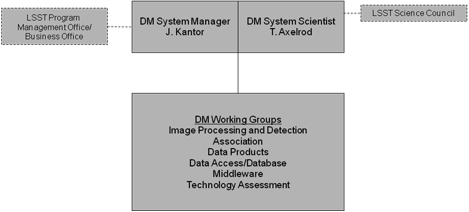
\includegraphics[width=0.8\textwidth]{images/precon}
\caption{Data Management Conceptual Design Phase Organization\label{fig:precon}}
\end{center}
\end{figure}

\subsection{
Preliminary Design Phase
}
The organization transitions to a more complex structure during Preliminary Design, as the role of each DM partner institution is solidified, and D\&D prototype development projects called Data Challenges become a primary organizing/tasking vehicle for D\&D work.  The Working Groups still remain and play a cross-institutional functional role in each area, but there is a more formal structure for work allocation and responsibility, as shown in \figref{fig:pdphase}.



\begin{figure}[htbp]
\begin{center}
 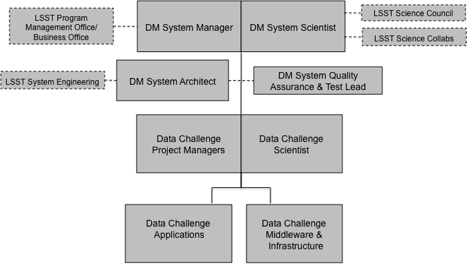
\includegraphics[width=0.8\textwidth]{images/pdphase}
\caption{ Data Management Preliminary Design Phase Organization\label{fig:pdphase}}
\end{center}
\end{figure}


In this phase, new positions reporting to the Project Manager and Project Scientist are added.  First, there is the DM System QA and Test Lead, who assists the Project Manager in preparation of formal plans, processes, and environments for software development, integration, and test. 
A Data Management System Architect supports the Project Manager and Project Scientist in matters related to LSST system engineering, including other subsystem interfaces, overall LSST system control, real-time external system interfaces (e.g. alerting), simulation, and end-to-end system engineering for quality assessment.
Finally, temporary Data Challenge Teams consisting of astronomers and engineers are formed for prototyping specific critical design aspects that have high risk (e.g. precursor and simulated data processing and prototype work, research and development of new algorithms for moving object detection or data distribution).  Each Data Challenge Team has a designated Project Manager who reports to the Project Manager and Scientist who reports to the Project Scientist for the duration of the Data Challenge.


\subsection{
Final Design Phase
}
During Final Design Phase, the organization structure transitions to one that will persist for the remainder of the period in which the DM System is developed and commissioned, up to the start of LSST Observatory operations.
As shown in \figref{fig:fdphase}, the organization now features lead institutions, each with responsibility for major element of the DM System (Level 2 Work Breakdown Structure elements) and Project Manager.  For example, during Final Design, the Processing Services/Tools and Archive Site Manager and Team at NCSA will be conducting prototyping activities in computing, data communications, and data storage to select and verify the ability of System technologies to support the LSST requirements.  They will also be involved in creating a supporting infrastructure for the DM Systems.  During Construction before the LSST first light time frame, these resources will be focused on implementation of the selected technologies.  In order to ensure that team functions as one integrated project, the institutions coordinate support by other lead institution team members directly through this organizational structure, as well as via a number of cross-organizational bodies (described later in this document). 
Also, due to the span of the organization, the DM Project Manager will be supported by one of the lead institution Project Managers as a Deputy Project Manager in these phases.


\begin{figure}[htbp]
\begin{center}
 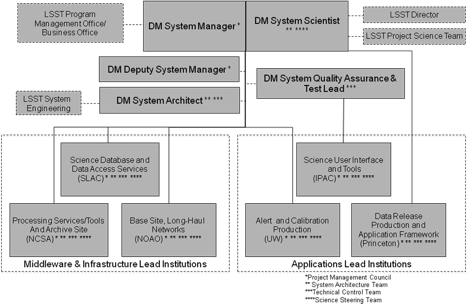
\includegraphics[width=0.8\textwidth]{images/fdphase}
\caption{ Data Management Final Design Phase Organization\label{fig:fdphase}}
\end{center}
\end{figure}



